\begin{center}{ \bf  ГИДРОДИНАМИЧЕСКИЙ
ПОДХОД К МОДЕЛИРОВАНИЮ РАСПРЕДЕЛЕНИЯ ИНВЕСТИЦИЙ}\\
{\it О.В. Владимирова} \\
(Воронеж; {\it olga\_vladimirova95@mail.ru} )
\end{center}
\addcontentsline{toc}{section}{Владимирова О.В.}


1. Одним из ключевых вопросов экономической динамики является
объяснение механизмов {\em рождения} и {\em распространения}
инноваций. По мнению многих аналитиков, эти два механизма лежат в
основе доминирования Западной цивилизации. Без интенсивного рождения
инноваций Западный мир не смог бы обогнать Восток в лице Китая и
Индии, и без бурного накопления капитала и инвестирования в
распространение новых технологий Запад не смог бы обеспечить своего
тотального превосходства [1]-[3]. Таким образом, вопрос о механизмах
рождения и распространения инноваций имеет цивилизационное значение.
Выяснение закономерностей рождения и распространения технологических
инноваций позволяет объяснить многие экономические явления.
Например, известное уравнение Пол\-те\-ро\-ви\-ча-Хен\-ки\-на
позволяет достаточно точно описывать эволюцию распределения
предприятий по уровням технологической эффективности, но оставляет
без ответа, например, вопрос о причине перехода предприятий к той
или иной инновационной стратегии. Почему одни предприятия переходят
к заимствованию более эффективной технологии, а другие - нет? Почему
одни это делают быстрее, а другие - медленнее? В уравнении
Полте\-ро\-ви\-ча-Хен\-ки\-на нет соответствующих переменных, на
основе которых можно было бы бы пояснить возникающие эффекты.

Специалисты считают, что механизм эволюции, зало-
\linebreak
женный в модель
Полтеровича-Хенкина, слишком прост, а само уравнение относится к
классу феноменологических моделей. Существующая аналогия между
уравнением Пол\-те\-ро\-ви\-ча-Хен\-ки\-на и уравнением Бюргерса [4]
является чисто формальной, ибо турбулентный процесс, описываемый
уравнением Бюргерса, совершенно не похож на процесс <<перетекания>>
предприятий по разным технологиям, описываемый уравнением
Полтеровича-Хенкина. С другой стороны, модель
Полтеровича-Хен\-ки\-на показывает глубокую аналогию экономических
процессов с физическими. Посредством этого уравнения можно описать
волну распределения предприятий по технологическим уровням. Можно
даже наблюдать эффект <<бегущей волны>>, когда вдоль оси времени
перемещается горб распределения. Подобное перемещение гребня волны
равносильно ликвидации старых технологий и рождению новых. Все
технологические уровни, которые остаются позади гребня волны
<<вдавливаются>> в зону технологической дыры, тогда как технологии,
лежащие впереди гребня, <<поднимаются>> из технологической
сингулярности. Таким образом, бегущая волна является математическим
выражением технологического прогресса.

2. В настоящей заметке рассмотрен прямой подход к описанию влияния
технологической диффузии на распреление инвестиций, основанный на
гидродинамической аналогии. Пусть имеется фирма и или финансовая
компания, состоящая из  $n$ преприятий, и пусть при этом
$r=\left(r_1,\dots\,, r_n\right)^\top$ --- вектор инвестирования
инноваций в этой фирме ($r_j = r_j(t)$  --- капитальные затраты на
инновации $j$-го предприятия вплоть до момента времени $t$), \
$v=\left(v_1,\dots\,, v_n\right)^\top$ --- вектор скорости
инвестирования инноваций ($v_j = \dot{r}_j$), \ а
$s=\left(s_1,\dots\,, s_n\right)^\top\in\Omega$ --- вектор
внедренных инноваций к данному моменту времени (например, в
процентах от планового показателя внедрения инноваций за весь
контрольный период). Будем предполагать, что выполнено следующее
условие: {\em вектор скорости внедрения инноваций пропорционален
вектору скорости инвестиций}: $\dot s = \beta v$ \ ($\beta$ ---
${\rm const}$). При выполнении этого условия поток инвестирования
инноваций <<параллелен>> потоку внедренных инноваций, то есть
рассчитав поток реализованных инвестиций, мы автоматически получаем
и поток внедренных инноваций. Для поля скоростей инвестирования
можно составить балансовое уравнение. Сначала заметим, что
 $
\frac{dv}{dt} = \dot{v} + \frac{\partial v}{\partial r}\,\dot{r} =
\dot{v}  + \frac{\partial v}{\partial r}\,v
 $
(здесь $\frac{\partial v}{\partial r} = \left(\frac{\partial
v_j}{\partial r_k}\right)$ --- матрица Якоби). Следовательно,
уравнение динамики инвестирования инноваций можно записать в виде,
аналогичном широко известному уравнению Навье-Стокса из динамики
несжимаемой вязкой жидкости [5]:
 $
\dot{v}  + \frac{\partial v}{\partial r}\,v = \mu \, \Delta(v) -
{\rm grad}\, (p) \,,
 $
где $v = v(r,t)$\,, \ $p = p(r,t)$--- функция влияния спроса и
предложения на инновации (инновационный потенциал), $\Delta =
\sum\limits_{j=1}^n \frac{\partial^2}{\partial r_j^2} $ ---
$n$-мерный гармонический оператор. Слагаемое $\mu \, \Delta(v)$ в
последнем уравнении отвечает за диффузию инвестиций (вызванную
диффузией инноваций), коэффициент \ $\mu$ \ характеризует <<
инновационную вязкость>> [6]. Естественно предположить также, что
выполнено условие неразрывности
 $
{\rm div}(v) = 0
 $
и граничное условие
 $
(v,n)\big |_{\partial \Omega} = 0\,
 $
на границе области $\Omega \,: = \{r =\left(r_1,\dots\,,
r_n\right)^\top\big | \ 0 \le r_j \le R_j\}$, \ $R_j$ --- потолок
инвестирования инноваций на $j$-ом предприятии, $n$ --- нормаль к
примыкающей максимальной грани границы.

Для повышения точности модели Бюргерса [5] (как одномерного варианта
классического уравнения Навье-Сток\-са) можно ввести дополнительное
слагаемое $v\,\left(\lambda\, - \|v\|^2\right)$, учитывающeе прямой
(механический) обмен инновационными ресурсами (см. [7]). В
результате получим обобщенное модельное уравнение в виде
 $
\dot{v} + \frac{\partial v}{\partial r}\,v = \mu \, \frac{\partial^2
v}{\partial r^2} + v\,\left(\lambda - \|v\|^2\right) - c \,.
 $
Анализ решений этого уравнения  базируется на вычислении собственных
функций и собственных значений операторного пучка  $A + \lambda\,B :
E \to F$ , \ $A = \frac{d^4}{dx^4}$\,, \ $B = \frac{d^2}{dx^2}$ (в
одномерном случае) при краевых условиях Дирихле и Неймана,\  $E = \{u
\in C^4 [0,1]: u(0)=u(1)=u'(0)=u'(1) = 0 \}$, $ F = C[0,1]$.
Собственные функции операторного пучка $A +\lambda\,B$ в
пространстве $E$ определяются формулой
 $
u_k(r)=1-\cos(2\,k\,r)\,,
 $
отвечая собственному значению $\lambda=4(\pi\,k)^2\,$ . Приближение
Бубнова-Галеркина по $n$ модам к решению уравнения Бюргерса имеют
следующий вид:
 $
v(r,t) = \sum\limits_{k=1}^n\,\xi_k(t)u_k(r)\,.
 $
Поток инвестиций определяется дифференциальным уравнением
 $
\dot r=v(r,t)\,.
 $
Для $n=1,2,3$ при определенных начальных данных получаются графики
инвестиционных поступлений в следующем виде:

\begin{figure}[h!t]
	\centering
	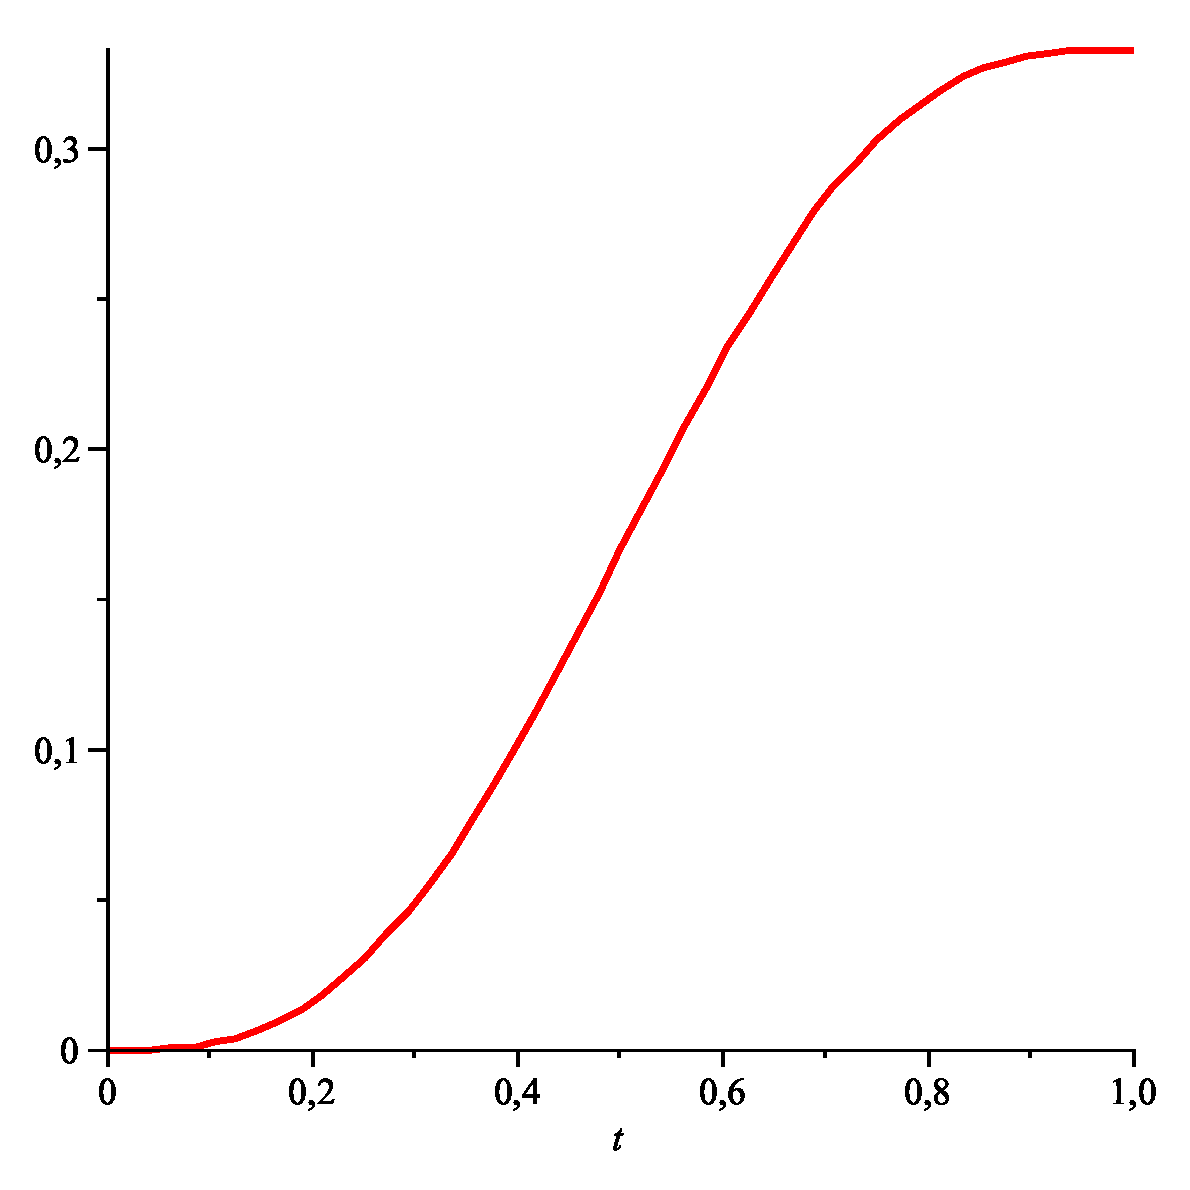
\includegraphics[width=0.2\textwidth,angle=0]{1mod.eps} \ \ \
	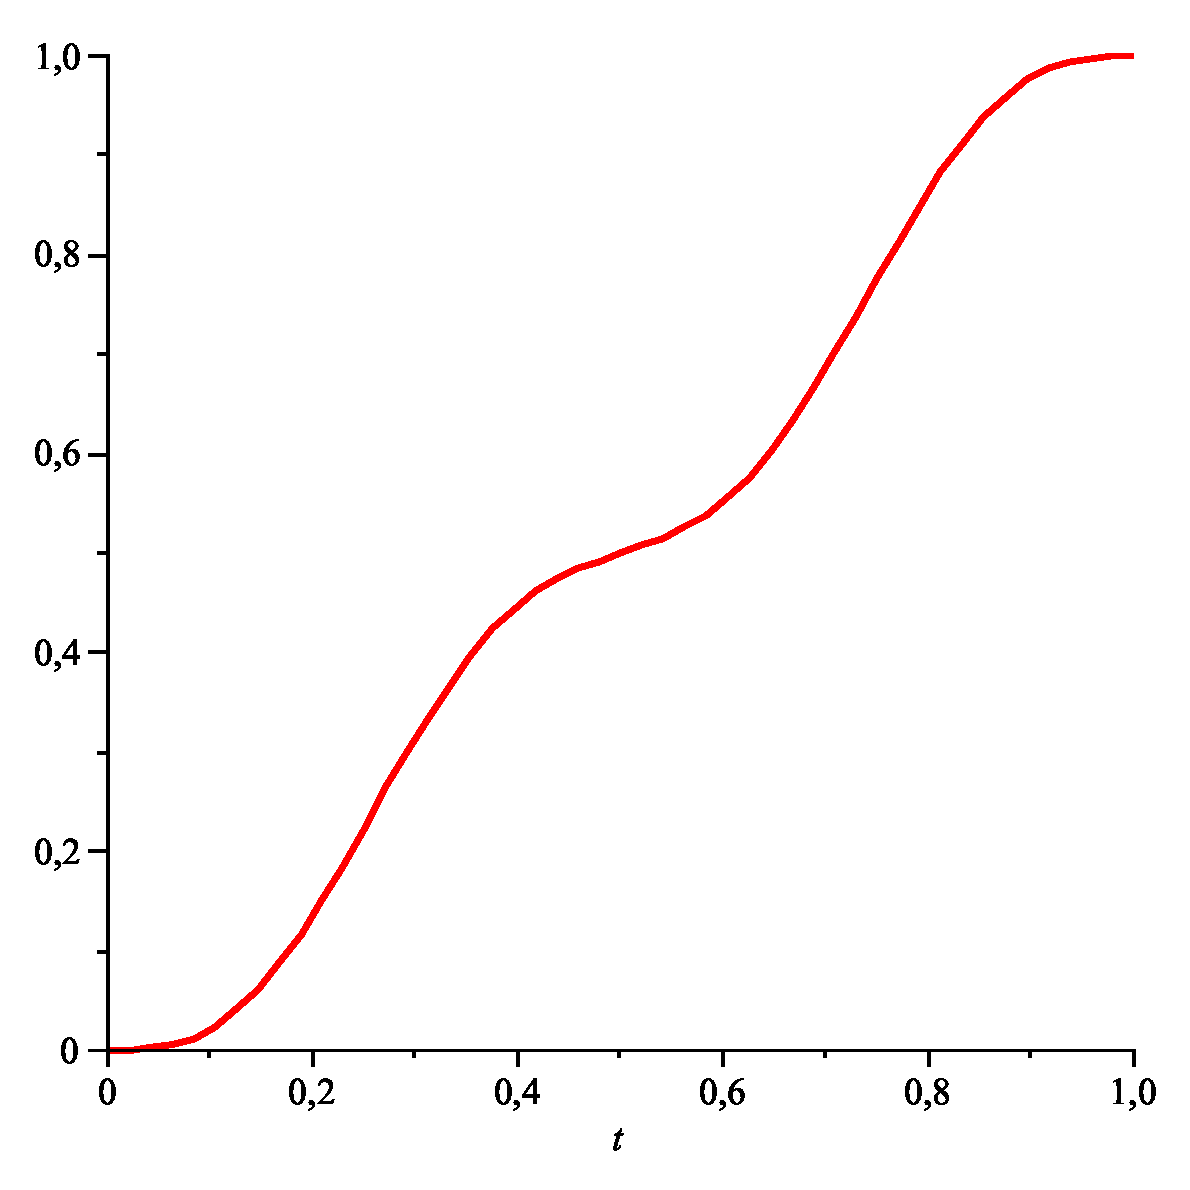
\includegraphics[width=0.2\textwidth,angle=0]{2mod.eps} \ \ \
	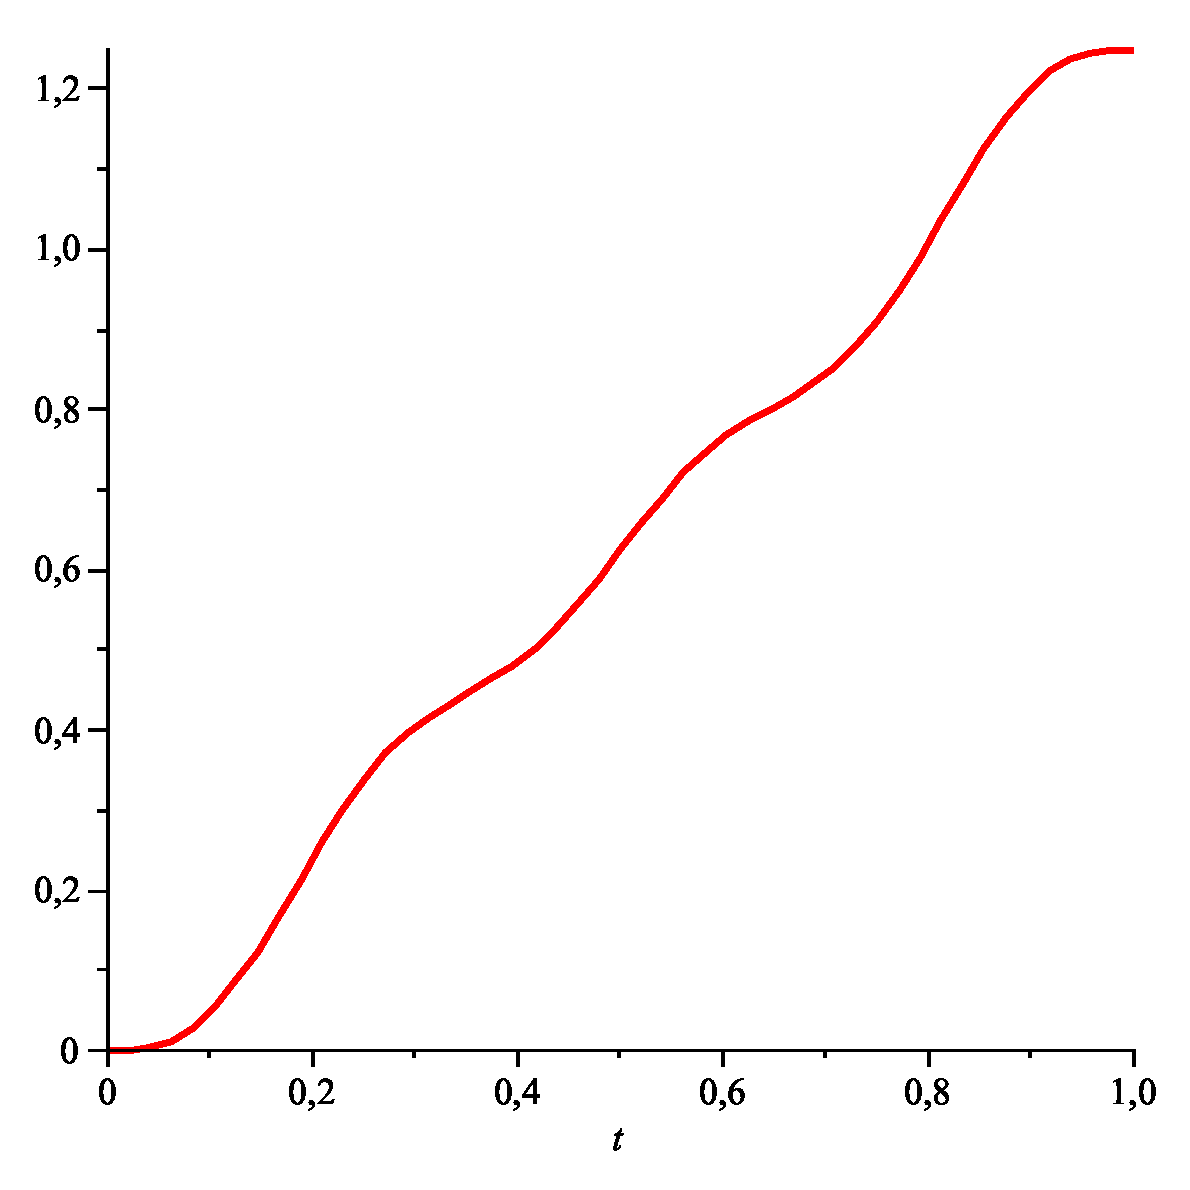
\includegraphics[width=0.2\textwidth,angle=0]{3mod.eps}
	%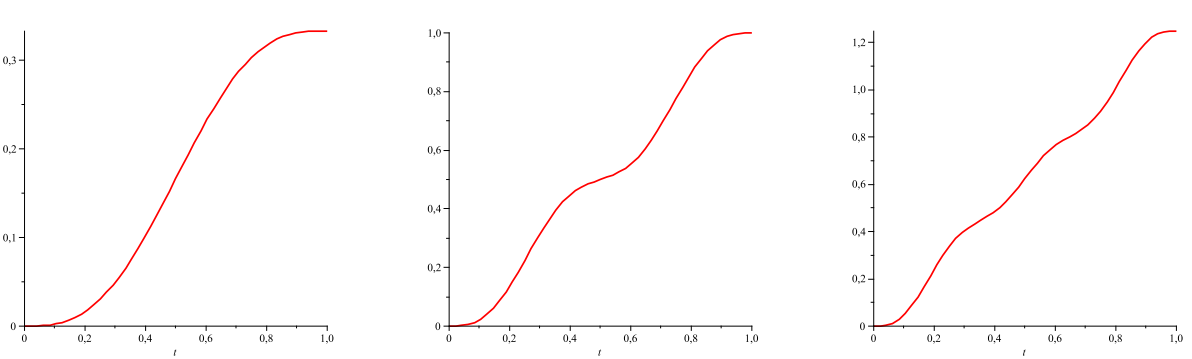
\includegraphics[width=1\textwidth]{Vladimirova_prtscr.png}
	\caption{
		Графики приближенно вычисленной функции
		инвестиций (аппроксимации Галеркина по одной, двум и трем модам) при
		некоторых начальных данных
	}
\end{figure}



3. Случай фирмы из двух преприятий. Пусть
 $
n=2\, \ \ r=\left(r_1, r_2\right)^\top, \ \ v=\left(v_1,
v_2\right)^\top, \ \ s=\left(s_1,s_2\right)^\top\,,
 $
 $
\Omega\,:= \,  \{0 \le r_1 \le 1\,, \ 0 \le r_2 \le 1\}\,.
 $
Рассмотрим случай стационарного уравнения :\ $\dot v \equiv 0$\,
вместе с  требованием выполнения краевого условия Дирихле (<<условия
прилипания>> на границе). Обратимся к двумерному уравнению
Навье-Стокса
  $
\dot v + \frac{\partial v}{\partial r}\,v = \mu\Delta (v) - {\rm
grad}\,(p)
  $
при краевом условии Дирихле. Здесь $\Delta$ --- двумерный
гармонический оператор (лапласиан), $\frac{\partial v}{\partial r}$
--- матрица Якоби вектора скорости $v=v(r,t)$ инновационного
потока по компонентам $r=(r_1,r_2)$\,, \ $p=p(r_1,r_2)$ ---
потенциал. Перейдем к другой форме уравнения, используя
нижеуказанные равенства (непосредственно устанавливаемые проверкой):
  $
{\rm rot}\left(\frac{\partial v}{\partial r}\right)={\rm
grad}\,(\Delta \psi);
 $
 $ \ {\rm rot}\left(\frac{\partial
v}{\partial r}\, v\right)=[\psi,\Delta (\psi)]\,,
  $
$ {\rm rot}\,(v) := \frac{\partial v_2}{\partial r_1}-\frac{\partial
v_1}{\partial r_2}\,, $ $\psi (r_1,r_2,t)$ --- вихревая функция,
$[\psi,\,\varphi]$ --- якобиан функций $\psi,\,\varphi$\,. Причем $
{\rm div}(v) =0 $ (условие неразрывности в односвязной области)
приводит к тому, что решение должно иметь вид:
 $
v = {\rm sgrad}(\psi) := \left(\frac{\partial\psi}{\partial
r_2}\,,\,-\frac{\partial\psi}{\partial r_1}\right)^\top\,.
 $
Из краевого условия для $v$ следует выполнение для функции $\psi$
граничного условия
  $
({\rm grad}(\psi),\tau)\,\bigg |_{\partial \Omega} = 0\,,
  $
где $\tau$ --- касательный к $\partial \Omega$ вектор.
Следовательно, $ \psi\bigg |_{\partial \Omega} = {\rm const}\,.$
Положим
 $
\psi\bigg |_{\partial \Omega} = 0\,
 $
(краевое условие Дирихле). Из граничного условия вытекает
соотношение
 $
\frac{\partial \psi}{\partial n}\bigg |_{\partial \Omega} = 0
  $
(краевое условие Неймана). Пусть $ u := {\rm rot}(v) = \Delta(\psi)$
и $ \dot u = {\rm rot}(\dot{v})=\Delta(\dot\psi). $ Применив
двумерный ротор к правой и левой частям уравнения получим уравнение
Гельмгольца (см. [6])
 $
\Delta(\dot\psi) = [\Delta(\psi),\,\psi] + \mu\,\Delta^2(\psi)
 $
и его стационарный вариант
 $
[\Delta(\psi),\,\psi] + \mu\,\Delta^2(\psi) = 0 \,.
 $
В случае обобщенного уравнения Навье-Стокса  получим обобщенное
стационарное уравнение Гельмгольца
 $
\mu\,\Delta^2(\psi) + \lambda\,\Delta(\psi) + [\Delta(\psi),\,\psi]
- \mathcal{B}^{(3)}(\psi) = 0 \,,
 $
где
 $
\mathcal{B}^{(3)}(\psi) = \psi_{r_1}^2\,\psi_{r_1r_1}+
\psi_{r_2}^2\,\psi_{r_2r_2}+
2\,\psi_{r_1}\psi_{r_2}\,\psi_{r_1r_2}\,,
 $ или
 $
\mathcal{B}^{(3)}(\psi)= \left(H(\psi)\,{\rm grad}\,(\psi) , {\rm
grad}\,(\psi)\right)\,,
 $
$H(\psi):= (\psi_{r_jr_k})$ --- матрица Гессе вихревой функции.


\begin{center}

{\bf Литература}

\end{center}

1. Гельман Л.М., Левин М.И. Модели инновационных процессов (обзор
зарубежной литературы) / Л.М. Гельман,  М.И. Левин // Экономика и
математические методы, \No 6, 1989.

2. Полтерович В.М. Эволюционная модель взаимодействия процессов
создания и заимствования технологий /
\linebreak
В.М. Полтерович, Г.М. Хенкин
// Экономика и математические методы, №6, 1988.

3. Гельман Л.М. Моделирование динамики распределения предприятий
отрасли по уровням эффективности (на примере черной металлургии) /
Л.М. Гельман, М.И. Левин, В.М. Полтерович, В.А. Спивак // Экономика
и математические методы, №3, Том 29, 1993.

\selectlanguage{english}

4. Burgers J.M. A mathematical model illustrating the theory of
turbulence / J.M. Burgers // Advances in Applied Mechanics. Ed.
R.V.Mises and T.V.Karman. 1948.

\selectlanguage{russian}

5. Ландау Л.Д. Теоретическая физика. Т. VI. Гидродинамика / Л.Д.
Ландау, Е.М. Лифшиц //  М.: Наука. 1986. - 736 с.

6. Сапронов Ю.\,И. Гидродинамический подход к моделированию
инновационного потока / Ю.\,И. Сапронов,
\linebreak
О.\,В.~Владимирова, В.\,А.
Иванюхин, В.\,В. Конев // Материалы межд. конф. "ВЗМШ С.Г. Крейна -
2016". ИПЦ "Научная книга", 2016. - С. 342-350.

7. Арнольд В.И. «Жёсткие» и «мягкие» математические модели. – 2-е
изд. стереотип. / В.И. Арнольд // М.: МЦНМО, 2008. - 32 с.
